\begin{frame}
  \frametitle{The Cosmic Microwave Background}

  \begin{overlayarea}{\textwidth}{\textheight}

    \only<1-2>{%
      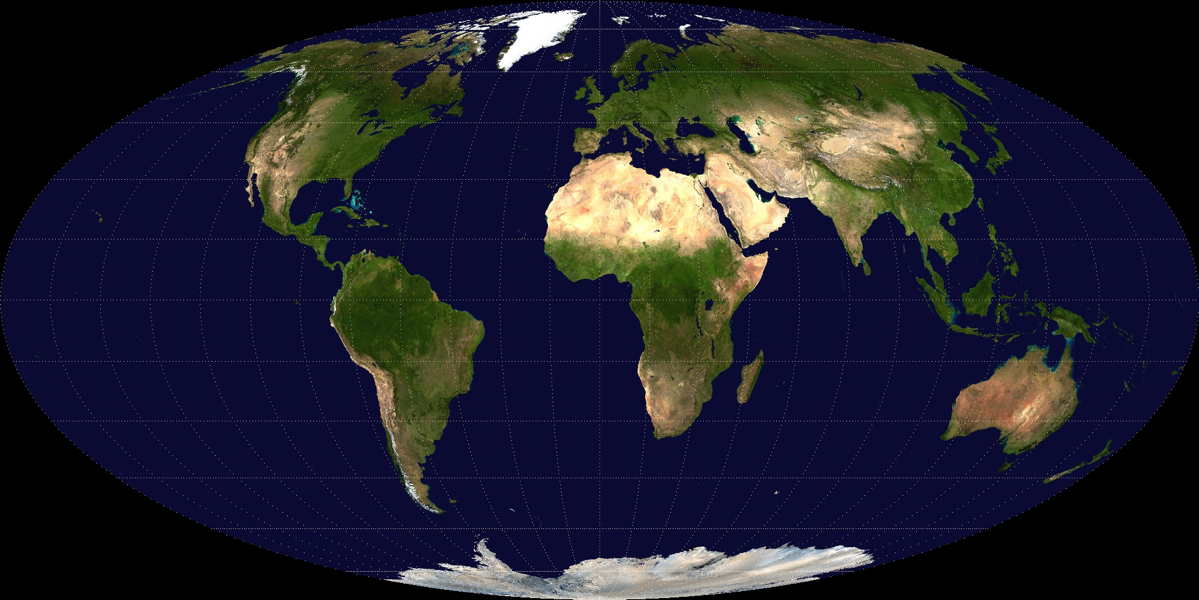
\includegraphics[width=\textwidth]{Images/Mollweide-projection.png}
    }
    \only<3-4>{%
      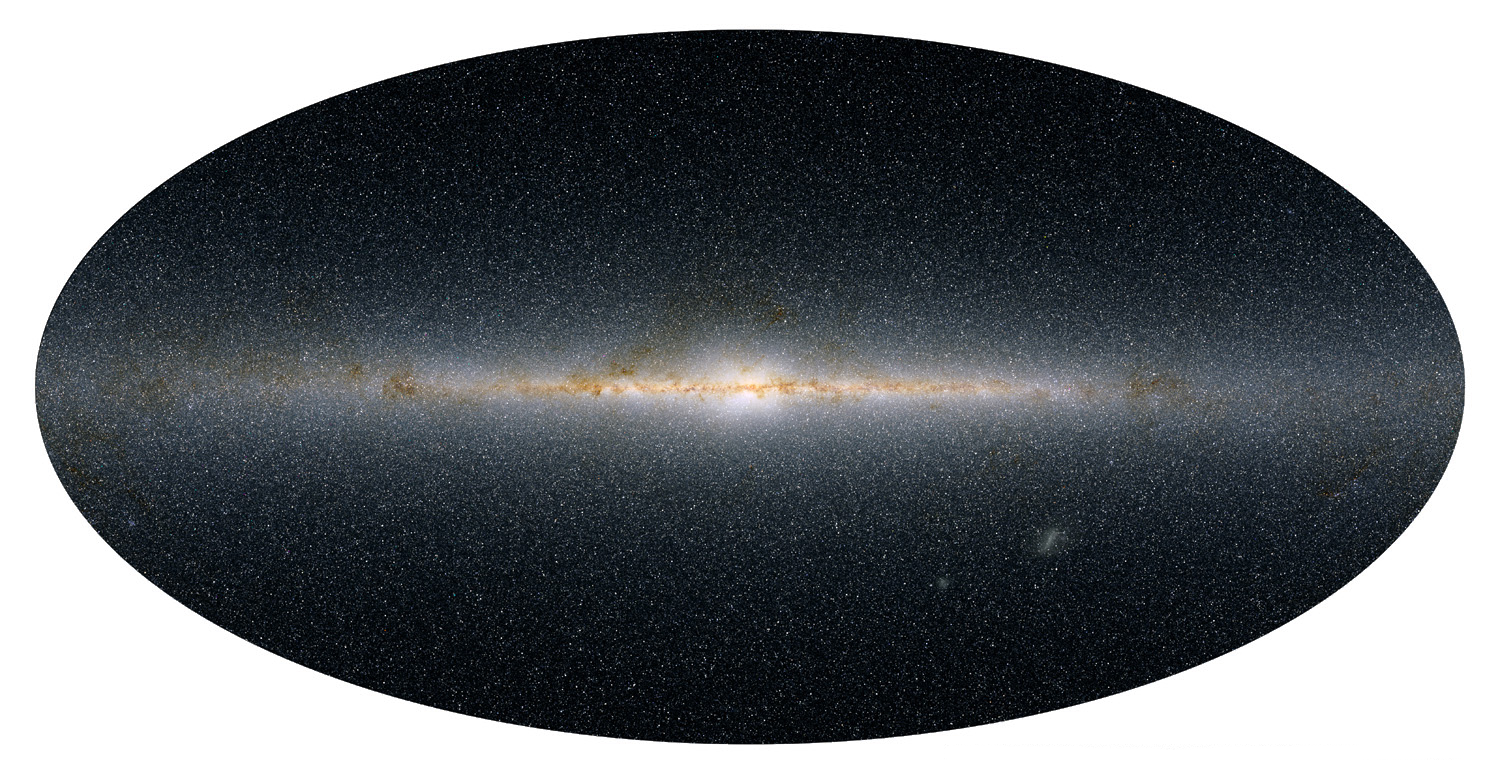
\includegraphics[width=\textwidth]{Images/Milky_Way_infrared.png}
    }
    \only<5->{%
      
\includegraphics[width=\textwidth]{Images/monopole.jpg}
    }

    \begin{itemize}
      \only<1-2>{\item A map of the Earth (Mollweide projection).}
      \only<2-2>{\item Consider the same map, but looking out at the night sky.}
      \only<3-4>{\item This image is taken in the infra-red waveband.}
      \only<4-5>{\item Now look in the microwave band.}
      \only<6- >{\item The sky is filled with the Cosmic Microwave Background radiation (CMB).}
      \only<7- >{\item The CMB has a temperature of $2.7260$ K.}
      \only<8- >{\item It is {\em too\/} uniform.}
    \end{itemize}

  \end{overlayarea}
\end{frame}
